\newpage
\section{Thực hành nhóm}
\subsection{Yêu cầu}
Thực hiện chương trình tính tích vô hướng của 2 vector.
\subsection{Cơ sở toán học}
Tích vô hướng của 2 vector là một phép toán đại số và cho kết quả là một số vô hướng, được tính bằng cách lấy tổng của tích từng cặp phần tử tương ứng:

\[ \mathbf{u} \cdot \mathbf{v} = \sum_{i=1}^{n} u_i \cdot v_i \]

Trong đó:


\begin{itemize}
 \item Với \( \mathbf{u} \) và \( \mathbf{v} \) là hai vector có cùng số chiều \( n \).
 \item Với \( u_i \) và \( v_i \) là phần tử thứ \( i \) của \( \mathbf{u} \) và \( \mathbf{v} \) tương ứng.
\end{itemize}

\textbf{Ví dụ:}

Cho 2 vector \( \mathbf{u} = \langle 1, 2, 3 \rangle \) và \( \mathbf{v} = \langle 4, 5, 6 \rangle \), thì tích vô hướng của \( \mathbf{u} \) và \( \mathbf{v} \) là:

\[ \mathbf{u} \cdot \mathbf{v} = 1 \cdot 4 + 2 \cdot 5 + 3 \cdot 6 = 42\]






\subsection{Mã nguồn tính tích vô hướng của 2 vector}

\subsubsection{Mã nguồn tạo vector ngẫu nhiên}
\begin{listing}[H]
 \centering
 \inputminted{cpp}{sources/MaNguon2NN.cpp}
 \caption{Mã nguồn tạo vector ngẫu nhiên}
 \label{code:MaNguon2NN}
\end{listing}



\subsubsection{Mã nguồn lập trình tuần tự tính tích vô hướng của 2 vector}
\begin{listing}[H]
 \centering
 \inputminted{cpp}{sources/MaNguon2TT.cpp}
 \caption{Mã nguồn lập trình tuần tự tính tích vô hướng của 2 vector}
 \label{code:MaNguon2TT}
\end{listing}




\subsubsection{Mã nguồn lập trình song song tính tích vô hướng của 2 vector}
\begin{listing}[H]
 \centering
 \inputminted{cpp}{sources/MaNguon2SS.cpp}
 \caption{Mã nguồn lập trình song song tính tích vô hướng của 2 vector}
 \label{code:MaNguon2SS}
\end{listing}

Trong mã nguồn sử dụng \texttt{\#pragma omp parallel for reduction(+ : result)} là một chỉ thị được sử dụng trong OpenMP với ý nghĩa:

\begin{enumerate}
 \item \texttt{\#pragma omp}: thông báo cho trình biên dịch hiểu rằng phần mã nguồn sau đó sẽ được thực hiện theo kiểu lập trình đa luồng của OpenMP.

 \item \texttt{parallel for}: thông báo cho trình biên dịch sử dụng đa luồng cho các lần lặp của vòng lặp \texttt{for} tiếp theo.

 \item \texttt{reduction(+ : result)}: sử dụng để chỉ định một toán tử cụ thể. Khi một toán tử được chỉ định, mỗi luồng duy trì một bản sao riêng tư của biến và cuối vùng song song, các kết quả được kết hợp bằng cách sử dụng toán tử đã được chỉ định. Trong mã nguồn này, là phép cộng (\texttt{+}) trên biến \texttt{result}.
\end{enumerate}

Trong ví dụ này, vòng lặp được lập trình đa luồng, và mỗi luồng đóng góp vào tổng của \texttt{result}. Cuối cùng, các kết quả cá nhân của luồng được kết hợp, và tổng cuối cùng được in ra màn hình.








\newpage
\subsection{Kết quả:}
\subsubsection{Bảng kết quả tính tích vô hướng của 2 vector}


 
 \begin{table}[h] %!nghia
 \centering
 \begin{tabular}{|c|c|c|c|}

 \hline
 \multicolumn{3}{|c|}{\textbf{BẢNG KẾT QUẢ}} \\ 
 \hline
 \textbf{Kích thước} & \textbf{Thời gian lập trình tuần tự} & \textbf{Thời gian lập trình song song} \\ \hline
 11111111111111111 & 11111111111111111 & 11111111111111111 \\ \hline
 11111111111111111 & 11111111111111111 & 11111111111111111 \\ \hline
 11111111111111111 & 11111111111111111 & 11111111111111111 \\ \hline
 \end{tabular}

 \caption{ViDuBangThuong} %!nghia
 \label{table:nghia123} %!nghia
 \end{table} 



\newpage
\subsubsection{Biểu đồ tính tích vô hướng của 2 vector}


 
\begin{figure}[h] %!nghia
\centering
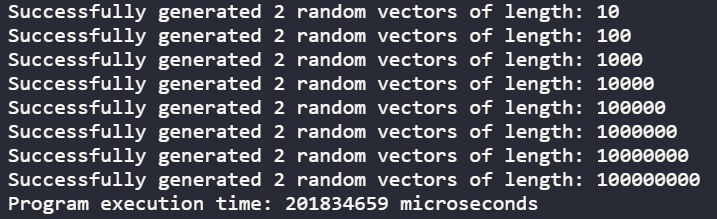
\includegraphics[width=1\textwidth]{pictures/image.png} %!nghia
\caption{ViDuHinhAnhTheoChieuNgang} %!nghia
\label{pictures:nghia1} %!nghia
\end{figure} 






\subsection{Nhận xét}
\lipsum[1]